\posl{} permet de construire des solveurs suivant différentes étapes : 
\begin{enumerate}
\item  L'algorithme du solveur considéré est  exprimé via une décomposition  en modules de calcul. Ces modules sont implémentés à la   manière de {\it fonctions} séparées. Nous appelons \infr{\om{}} ces morceaux de calcul (figure \ref{res_subfig:modules}, blocs bleus). En suite, il faut décider  quelles sont les types d'informations que l'on souhaite recevoir des autres solveurs. Ces informations sont encapsulées  dans des composants appelés \infr{\opch{}},  permettant de transmettre des données entre solveurs (figure \ref{res_subfig:modules}, bloc rouge) \label{res_stages:module}

\item  Une {\it stratégie générique}  est codée  à travers  \posl{}, en utilisant les  opérateurs fournis par le langage appliqués  sur des modules \textit{abstraites} qui représentent les \textit{signatures} des composants donnés lors de l'étape 1, pour créer des \infr{\ass}. Cette stratégie définit non seulement les informations échangées, mais détermine également l'exécution parallèle de composants. Lors de cette  étape, les informations à partager sont  transmises via les opérateurs \textit{ad-hoc}. On peut voir cette étape comme la définition de la colonne vertébrale des solveurs (figure \ref{res_subfig:as}).

\item  Les solveurs sont créés en instanciant l'\infr{\as}, par \infr{\oms{}} et \infr{\opchs}. %puis en les assemblant 

\item Les solveurs sont assemblés en utilisant les opérateurs de communication fournis par le langage, pour créer des stratégies de communication. Cette entité finale s'appelle \infr{\soset{}} (figure \ref{res_subfig:comm}).
\end{enumerate}

\begin{figure}
	\centering
	\subfloat[][Définition des \infr{\oms} et les \infr{\opchs}]{
		\label{res_subfig:modules}
		
\includegraphics[width=0.3\columnwidth]{modules_1.png}
	}\\
	\subfloat[][Définition de l'\infr{\as}]{%
		\label{res_subfig:as}
		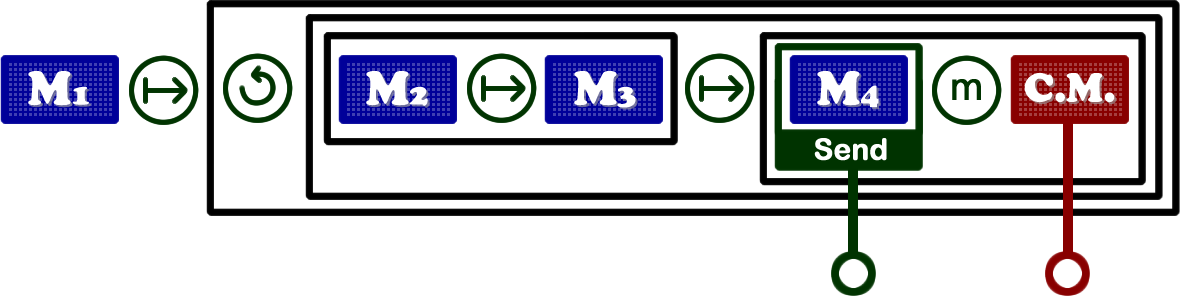
\includegraphics[width=0.5\columnwidth]{example_1.png}
	}\\
	\subfloat[][Définition de la stratégie de communication]{
		\label{res_subfig:comm}
		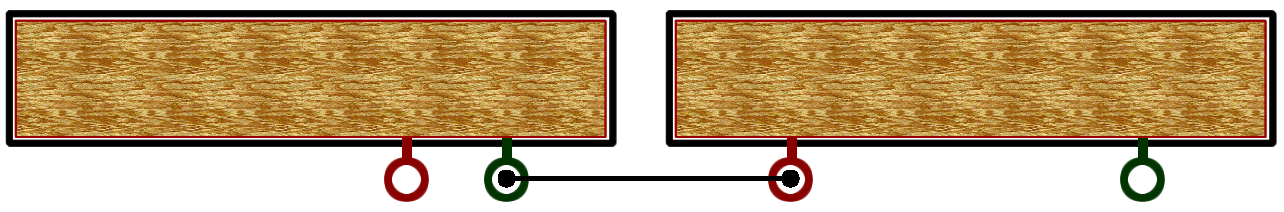
\includegraphics[width=0.6\columnwidth]{conn.png}
	}
	\caption[]{Construire des solveurs parallèles avec \posl{}}
	\label{res_fig:posl}
\end{figure}%fr

Les sous-sections suivantes expliquent en détail chacune des étapes ci-dessus.

\subsection{Computation module}

Un \infr{\om{}}  est la plus basique  et abstraite manière de définir un composant de calcul. Il reçoit une entrée, exécute un algorithme interne et retourne une sortie. Dans ce résumé, nous utilisons ce concept afin de décrire et définir les composants de base d'un  solveur, qui seront assemblés par l'\infr{\as}.  

Un \om{} représente un  morceau de l'algorithme du solveur  qui est susceptible de changer au cours de  l'exécution. Il peut être dynamiquement remplacé  ou combiné avec d'autres \infr{\oms}, puisque les \infr{\oms{}} sont également des informations échangeables  entre  les solveurs. De cette manière, le solveur  peut changer/adapter son comportement à chaud, en combinant  ses \infr{\oms{}} avec ceux  des autres solveurs. Ils sont  représentés par  des blocs  bleus dans  la figure~\ref{res_fig:posl}.

\begin{lemma}\label{res_def:module} \textbf{(Computation Module)}
Un \om{} $\mathcal{O}m$ est une application définie par :
\begin{equation}
 \mathcal{C}m:\mathcal{I} \rightarrow \mathcal{O}
\end{equation}
\end{lemma}

Dans (\ref{res_def:module}),  la nature de $\mathcal{D}$  et $\mathcal{I}$ dépend du type de \infr{\om{}}. Ils peuvent être soit une configuration, ou un  ensemble de configurations, ou un ensemble de valeurs de différents types de données, etc.

Soit une méta-heuristique de recherche locale, basée sur un algorithme bien connu, comme par exemple {\it Tabu Search}. Prenons l'exemple d'un  \infr{\om{}} retournant le voisinage d'une configuration donnée, pour une certaine métrique de voisinage. Ce \infr{\om{}} peut être défini par la fonction suivante:

\begin{equation}
\mathcal{C}m:D_1\times D_2\times\dots\times D_n \rightarrow 2^{D_1\times D_2\times\dots\times D_n}
\end{equation}

où $D_i$  représente  la  définition  des  domaines  de  chacune  des variables de la configuration d'entrée.

\subsection{Communication module}

Les \infr{\opchs{}} sont  les composants des solveurs en charge  de la réception des informations communiquées entre solveurs. Ils  peuvent interagir avec les \infr{\oms}, en fonction de l'\infr{\as}. Les \infr{\opchs{}} jouent le rôle de prise, permettant aux solveurs de  se  brancher et de recevoir des informations. Il sont représentés en rouge dans la figure~\ref{res_subfig:modules}.

Un \infr{\opch{}} peut recevoir deux types d'informations, provenant toujours d'un solveur tiers : des données et des \infr{\oms}. En ce qui concerne les \oms, leur communication peut se faire via la  transmission d'identifiants permettant à chaque solveur de les instancier.

Pour faire la distinction entre  les deux différents types de \infr{\opchs}, nous appelons \infr{\dopch{}} les \infr{\opchs{}} responsables de la réception de données et \infr{\oopch{}} ceux s'occupant de la réception et de l'instanciation de \infr{\oms}.

\begin{lemma} \label{res_def:dopench} \textbf{(\infr{Data communication module})}
Un \infr{\dopch{}} $\mathcal{C}h$ est un composant produisant une application définie comme suit : 
\begin{equation}
\mathcal{C}h: I\times\left\{D\cup\left\{NULL\right\}\right\} \rightarrow D \cup \left\{NULL\right\}
\end{equation}
et retournant l'information  $\mathcal{I}$ provenant d'un solveur tiers,quelque soit l'entrée $\mathcal{U}$.
\end{lemma}

\begin{lemma}\label{res_def:oopench} \textbf{(\infr{Object communication module})} 
Si nous notons $\mathbf{M}$ l'espace  de  tous  les \infr{\oms{}} de la définition~\ref{res_def:module}, alors un \infr{\oopch{}} $\mathcal{C}h$ est  un composant produisant un \infr{\om{}}  venant d'un solveur tiers défini ainsi :
\begin{equation}
\mathcal{C}h:I\times\left\{\mathbf{M}\cup\left\{NULL\right\}\right\} \rightarrow O\cup\left\{NULL\right\}
\end{equation}
\end{lemma}

Puisque les \infr{\opchs{}} reçoivent des informations provenant  d'autres solveurs sans pour autant avoir de contrôle sur celles-ci, il est  nécessaire  de définir l'information {\it  NULL}, signifiant l'absence  d'information. La figure~\ref{res_fig:ochperform}  montre  le mécanisme interne d'un \infr{\opch{}}. Si un \infr{\dopch{}} reçoit une information, celle-ci est automatiquement retournée (figure~\ref{res_subfig:doch}, lignes bleues). Si un \infr{\oopch{}} reçoit un \infr{\om{}}, ce dernier est instancié et exécuté avec l'entrée du \infr{\opch}, et le résultat est retourné (figure \ref{res_subfig:ooch}, lignes bleues). Dans les deux cas, si aucune information n'est reçue, le \infr{\opch{}} retourne l'objet  {\it NULL}  (figure \ref{res_fig:ochperform}, lignes rouges).

\begin{figure}
	\centering
	\subfloat[][\infr{Data \opch}]{
		\label{res_subfig:doch}
		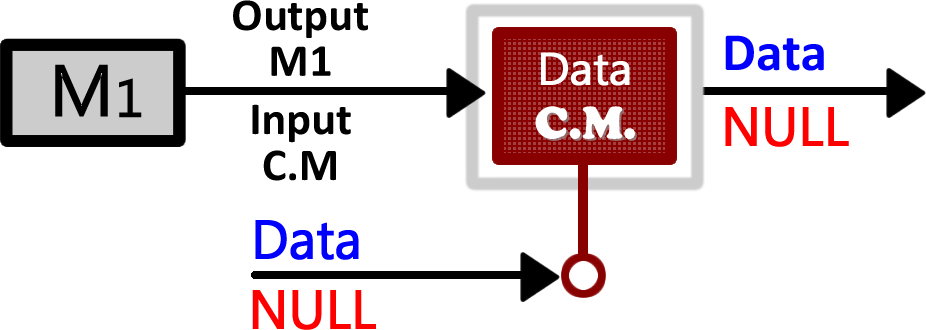
\includegraphics[width=0.4\linewidth]{D_OCh_v2.png} %[width=0.2\textwidth]{muta1}
	}
	\hspace{0.05\textwidth}%
	\subfloat[][\infr{Object \opch}]{%
		\label{res_subfig:ooch}
		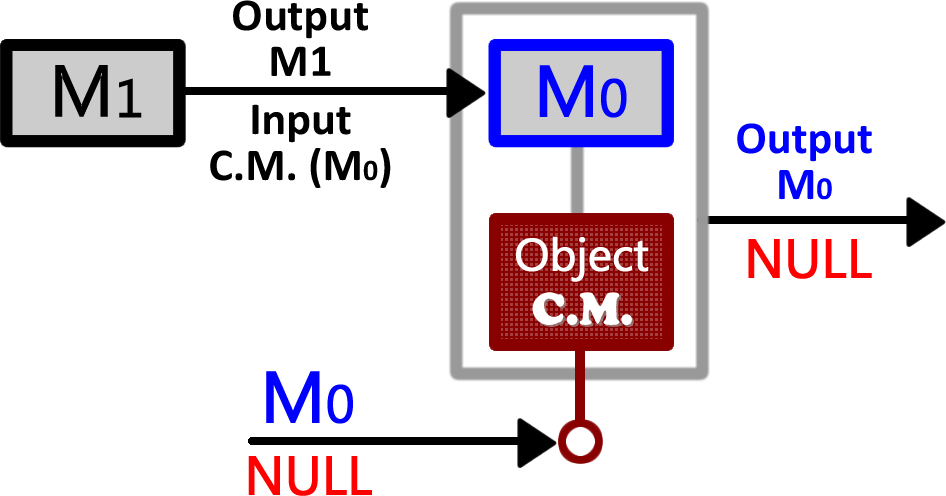
\includegraphics[width=0.4\linewidth]{O_OCh_v2.png}%[width=0.2\textwidth]{muta2}
	}
	\caption[]{Mécanisme interne du \opch}
	\label{res_fig:ochperform}
\end{figure}%fr

\subsection{Abstract solver}

L'\infr{\as{}} est le c\oe{}ur du solveur. Il joint les \infr{\oms{}} et les \infr{\opchs{}} de  manière cohérente, tout en leur restant indépendant. Ceci signifie  qu'il peut changer ou être modifié durant l'exécution, sans altérer  l'algorithme général et en respectant la structure du solveur. À travers l'\infr{\as}, on peut décider également des informations à envoyer aux autres solveurs. Chaque fois que nous combinons certains composants en utilisant des opérateurs \posl{}, nous créons un nouveau \infr{\m}.

\begin{lemma}
\label{res_def:cm}
Noté par la lettre $\mathcal{M}$, un {\bf \m} est:
\begin{enumerate}\renewcommand{\labelitemi}{\scriptsize$\blacksquare$}
\item un \infr{\om{}}; ou
\item un \infr{\opch{}}; ou
\item $\left[\mbox{OP } \mathcal{M}\right]$, la composition d'un module $\mathcal{M}$ exécutée séquentiellement, en retournant une sortie, en dépendant de la nature de l'opérateur unaire \emph{OP}; ou \label{res_subdef:seq_uni}
\item $\left[\mathcal{M}_1 \mbox{ OP } \mathcal{M}_2\right]$, la composition de deux modules $\mathcal{M}_1$ et $\mathcal{M}_2$ exécutée séquentiellement, en retournant une sortie, en dépendant de la nature de l'opérateur binaire \emph{OP}.\label{res_subdef:seq}
\item $\left[\mathcal{M}_1 \mbox{ OP } \mathcal{M}_2\right]$, la composition de deux modules $\mathcal{M}_1$ et $\mathcal{M}_2$ exécutée, en retournant une sortie, en dépendant de la nature de l'opérateur binaire \emph{OP}. Ces deux opérateurs vont être exécutes en parallèle si et seulement si \emph{OP} supporte le parallélisme, ou bien il lance une exception en cas contraire.\label{res_subdef:par}
\end{enumerate}
Nous notons par $\mathbf{M}$ l'espace des \infr{\ms}, et nous appelons \infr{\cms{}} la composition de \ms{} présentés en \ref{res_subdef:seq_uni} \ref{res_subdef:seq}, et/ou \ref{res_subdef:par}.
\end{lemma}

Pour illustrer la définition~\ref{res_def:cm}, la figure~\ref{res_fig:cm} montre graphiquement le concept de \cm.
\begin{figure}
	\centering
	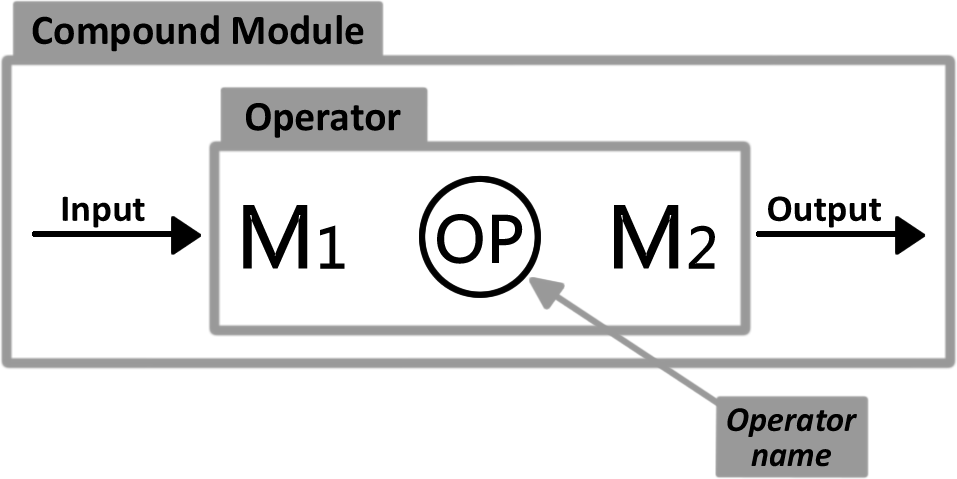
\includegraphics[width=0.4\linewidth]{cm.png} %[width=0.2\textwidth]{muta1}
	\caption[]{Un \infr{\cm}}
	\label{res_fig:cm}
\end{figure}%fr

Dans le cas particulier où un des \infr{\cms{}} impliqués est un \infr{\opch{}}, chaque opérateur gère l'information {\it NULL} à sa manière.

Afin de grouper des modules, nous utiliserons la notation $\left|.\right|$ comme un groupe générique qui pourra être indifféremment interprété comme $[.]$ ou comme $\lbk . \rbk_p$.

Ensuite, les opérateurs fournis par \posl{} sont présentés. 

\underline{\bf Sequential Execution Operator}: L'opération $\left|\mathcal{M}_1\poslop{\mapsto}\mathcal{M}_2\right|$ définit le \infr{\cm{}} $\mathcal{M}_{seq}$ comme le résultat de l'exécution de $\mathcal{M}_1$ suivi de $\mathcal{M}_2$. C'est un exemple d'opérateur ne  supportant pas une exécution en parallèle de ses \infr{\cms{}} impliqués, puisque l'entrée du second \infr{\cm{}} est la sortie du premier.

\underline{\bf Conditional Execution Operator}: L'opération $\left|\mathcal{M}_1\circled{?}_{<cond>}\mathcal{M}_2\right|$ définit le \cm{} $\mathcal{M}_{cond}$ le résultat de l'exécution en séquentiel de $\mathcal{M}_1$ si $<cond>$ est {\bf vrai} ou $\mathcal{M}_2$, autrement.

\underline{\bf Cyclic Execution Operator}: L'opération $\left|\circled{$\circlearrowleft$}_{<cond>}\mathcal{M}\right|$ définit le \cm{} $\mathcal{M}_{cyc}$ en répétant séquentiellement l'exécution de $\mathcal{M}$ tant que $<cond>$ est {\bf vrai}.

\underline{\bf Random Choice Operator}: L'opération $\left|M_1\circled{$\rho$}\mathcal{M}_2\right|$ définit le \cm{} $\mathcal{M}_{rho}$ qui exécute $\mathcal{M}_1$ en suivant une probabilité $\rho$, ou en exécutant $\mathcal{M}_2$ en suivant une probabilité $(1-\rho)$.

\underline{\bf Not {\it NULL}}: L'opération $\left|\mathcal{M}_1\circled{$\vee$}\mathcal{M}_2\right|$ définit le \cm{} $\mathcal{M}_{non}$ qui exécute $\mathcal{M}_1$ et retourne une sortie si elle n'est pas {\it NULL}, ou exécute $\mathcal{M}_2$ et retourne une sortie autrement.

\underline{\bf Minimum Operator}: Soient $o_1$ et $o_2$ les sorties de $\mathcal{M}_1$ et $\mathcal{M}_2$, respectivement. Nous assumons qu'il existe un ordre total dans $I_1 \cup I_2$ où l'objet \emph{NULL} est la plus grande valeur. Alors, l'opération $\left|\mathcal{M}_1\circled{m}\mathcal{M}_2\right|$ définit le \infr{\cm{}} $\mathcal{M}_{min}$ qui exécute $\mathcal{M}_1$ et $\mathcal{M}_2$, et retourne $\min\left\{o_1,o_2\right\}$.

\underline{\bf Maximum Operator}: Soient $o_1$ et $o_2$ les sorties de $\mathcal{M}_1$ et $\mathcal{M}_2$, respectivement. Nous assumons qu'il existe un ordre total dans $I_1 \cup I_2$ où l'objet \emph{NULL} est la plus petite valeur. Alors, l'opération $\left|\mathcal{M}_1\circled{M}\mathcal{M}_2\right|$ définit le \infr{\cm{}} $\mathcal{M}_{max}$ qui exécute $\mathcal{M}_1$ et $\mathcal{M}_2$, et retourne $\max\left\{o_1,o_2\right\}$.

\underline{\bf Race Operator}: L'opération $\left|\mathcal{M}_1\circled{$\shortdownarrow$}\mathcal{M}_2\right|$ définit le \infr{\cm{}} $\mathcal{M}_{race}$ qui exécute les deux \infr{\ms{}} $\mathcal{M}_1$ et $\mathcal{M}_2$, et retourne la sortie du \m{} qui termine en premier

Les opérateurs $\circled{$\rho$}$, $\circled{$\vee$}$ et $\circled{m}$ sont très  utiles en  terme de  partage d'informations entre   solveurs, mais également en terme de partage de comportements. Si un  des opérandes est un \infr{\opch{}} alors l'opérateur peut recevoir le \infr{\om{}} d'un autre solveur, donnant la possibilité d'instancier ce module dans le solveur le réceptionnant. L'opérateur va soit instancier le module s'il  n'est pas {\it NULL} et l'exécuter, soit exécuter le module donné par le second opérande.

Maintenant, nous présentons les opérateurs nous permettant d'envoyer de l'information vers d'autres solveurs. Deux types d'envois sont possibles :
\begin{inparaenum}[i)]
	\item on exécute un \infr{\m{}} et on envoie sa sortie,
	\item ou on envoie le \infr{\m{}} lui-même.
\end{inparaenum}

\underline{\bf Sending Data Operator}: L'opération $\left|\senddataop{\mathcal{M}}\right|$ définit le \infr{\cm{}} $\mathcal{M}_{sendD}$ qui exécute le \infr{\m{}} $\mathcal{M}$ puis envoie la sortie vers un \infr{\opch}.

\underline{\bf Sending Module Operator}: L'opération $\left|\sendmoduleop{\mathcal{M}}\right|$ définit le \infr{\cm{}} $\mathcal{M}_{sendM}$ qui exécute le \infr{\m{}} $\mathcal{M}$, puis envoie le \infr{\m{}} lui même  vers un \infr{\opch}.

Avec  les opérateurs  présentés jusqu'ici, nous sommes  en mesure  de concevoir les \infr{\ass{}} (ou algorithme) de résolution d'un problème de contraintes. Une fois un tel \infr{\as{}} défini, on peut changer les composants (\infr{\oms{}} et \infr{\opchs}) auxquels elle fait appel, permettant ainsi d'implémenter différents solveurs à partir du même \as{} mais composés de différents \infr{\ms}, du moment que ces derniers respectent la signature attendue, à savoir le types des entrées et sorties.

Un \as{} est déclaré comme suit: après déclarer les noms de l'\mbox{\tet{\bf \as}} ({\it name}), la première ligne définit la liste des \infr{\oms{}} abstraites ($\mathcal{L}^m$), la seconde ligne, la liste des \infr{\opchs{}} abstraites ($\mathbf{M}$), puis l'algorithme du solveur est définit comment le corps su solveur (le \infr{root \cm{}} $\mathbf{M}$), entre \mbox{\tet{\bf begin}} et \mbox{\tet{\bf end}}.

Un \as{} peut être déclaré par l'expression régulière suivante:

\begin{center}
\tet{\bf abstract solver} {\it name} \tet{\bf computation}: $\mathcal{L}^m$ (\tet{\bf communication}: $\mathcal{L}^c$)? \tet{\bf begin} $\mathbf{M}$ \tet{\bf end}
\end{center}

Par exemple, l'algorithme~\ref{res_algo:as_example} montre l'\infr{\as{}} correspondant à la figure~\ref{res_subfig:as}.

\begin{algorithm}[h]
\dontprintsemicolon
\scriptsize
\SetInd{2pt}{3pt}
\SetNoline
\SetKwProg{myproc}{}{}{}
\myproc{\tet{\bf abstract solver} as\_01\;
\tet{\bf computation} : $I, V, S, A$ \; 
\tet{\bf connection}: $C.M.$}{
	\Begin{
		$I \poslop{\mapsto}$
		\whileinline{$\left(\textbf{\Iter < } K_1\right)$}{
			$\left[V\poslop{\mapsto}S\poslop{\mapsto}\left[C.M.\poslop{m} \senddataop{A}\right]\right]$%
		}
	}
}
\caption{Pseudo-code \posl{} pour l'\infr{\as{}} de la figure~\ref{res_subfig:as}}\label{res_algo:as_example}
\end{algorithm}

\subsection{Créer les solveurs}

Maintenant on peut créer les solveurs en instanciant les \infr{\ms}. Il est possible de faire ceci en spécifiant qu'un \mbox{\tet{\bf solver}} donné doit implémenter (en utilisant le mot clé \mbox{\tet{\bf implements}}) un \as{} donné, suivi par la liste de \infr{\omprefix{}} puis \infr{\opchs{}}. Ces \ms{} doivent correspondre aux signatures exigées par l'\infr{\as}.

\begin{algorithm}[h]
\dontprintsemicolon
\scriptsize
\SetNoline
\SetKwProg{myproc}{}{}{}
\tet{\bf solver} solver\_01 \tet{\bf implements} as\_01\;
\tet{\bf computation} : $I_{rand}, V_{1ch}, S_{best}, A_{AI}$ \; 
\tet{\bf connection}: $CM_{last}$\;
\caption{Une instanciation de l'\as{} présenté dans l'algorithme~\ref{res_algo:as_example}}\label{res_algo:solver_def}
\end{algorithm}

\subsection{Connecter les solveurs : créer le \soset}

La dernière étape est de connecter les solveurs entre eux. \posl{} fournit des outils pour créer des stratégies de communication très facilement. L'ensemble des solveurs connectés qui seront exécutés en parallèle pour résoudre un CSP s'appelle \infr{\soset{}}.

Les communications sont établies en respectant les règles suivantes :
\begin{enumerate}
\item  À chaque  fois qu'un  solveur  envoie une information via les opérateurs  $\llparenthesis .\rrparenthesis^{d}$  ou $\llparenthesis   .\rrparenthesis^{m}$, il créé une {\it prise mâle de communication} 
\item À chaque fois qu'un  solveur contient un \infr{\opch{}}, il  crée une {\it prise femelle de communication} 
\item Les solveurs peuvent être connectés entre eux en reliant {\it prises mâles} et {\it femelles}.
\end{enumerate}

Avec l'opérateur~$(\posldot)$, nous  pouvons avoir accès aux \infr{\oms{}} envoyant une information et aux noms des \infr{\opchs{}} d'un solveur. Par exemple : $Solver_1\posldot\mathcal{M}_1$ fournit un accès au \infr{\om{}} $\mathcal{M}_1$ du $Solver_1$ si et seulement s'il est utilisé par l'opérateur  $\llparenthesis .\rrparenthesis^{d}$  (ou $\llparenthesis.\rrparenthesis^{m}$), et $Solver_2\posldot\mathcal{C}h_2$ fournit un accès au \infr{\opch{}} $\mathcal{C}h_2$ de $Solver_2$.

Maintenant, nous définissons les opérateurs de communication que \posl{} fournit.

\begin{lemma}\label{res_op_conn:1to1}
{\bf Opérateur de connexion \infr{\oneTone}} Soient
\begin{enumerate}
\item $\mathcal{J} = \left[\mathcal{S}_0\posldot \mathcal{M}_0, \mathcal{S}_1\posldot \mathcal{M}_1,\dots, \mathcal{S}_{N-1}\posldot \mathcal{M}_{N-1}\right]$ une liste de  {\it prises mâles}, et
\item $\mathcal{O} = \left[\mathcal{Z}_0\posldot \mathcal{CM}_0, \mathcal{Z}_1\posldot \mathcal{CM}_1,\dots, \mathcal{Z}_{N-1}\posldot \mathcal{CM}_{N-1}\right]$ une liste de {\it prises femelles}
\end{enumerate} Alors, l'opération
\[
\mathcal{J} \onetoonesep \mathcal{O}
\]
connecte chaque {\it prise mâle} $\mathcal{S}_i\posldot \mathcal{M}_i \in \mathcal{J}$ avec la {\it prise femelle} correspondante $\mathcal{Z}_i\posldot \mathcal{CM}_i \in \mathcal{O}$, $\forall\textbf{ }0 \leq i \leq N-1$ (voir figure~\ref{res_subfig:comm_simple}).
\end{lemma}

\begin{lemma}\label{res_op_conn:1ton}
{\bf Opérateur de Connexion \infr{\oneTn}} Soient 
\begin{enumerate} 
\item $\mathcal{J} = \left[\mathcal{S}_0\posldot \mathcal{M}_0, \mathcal{S}_1\posldot \mathcal{M}_1,\dots, \mathcal{S}_{N-1}\posldot \mathcal{M}_{N-1}\right]$ une liste de  {\it prises mâles}, et
\item $\mathcal{O} = \left[\mathcal{Z}_0\posldot \mathcal{CM}_0, \mathcal{Z}_1\posldot \mathcal{CM}_1,\dots, \mathcal{Z}_{M-1}\posldot \mathcal{CM}_{M-1}\right]$ une liste de {\it prises femelles}
\end{enumerate} Alors, l'opération
\[
\mathcal{J} \onetonsep \mathcal{O}
\]
connecte chaque {\it prise mâle} $\mathcal{S}_i\posldot \mathcal{M}_i \in \mathcal{J}$ avec chaque {\it prise femelle} $\mathcal{Z}_j\posldot \mathcal{CM}_j \in \mathcal{O}$, $\forall\textbf{ }0 \leq i \leq N-1$ et $0 \leq j \leq M-1$ (voir Figure~\ref{res_subfig:comm_diff}).
\end{lemma}


\posl{} permet aussi de déclarer des solveurs non communicatifs pour les exécuter en parallèle, en déclarant seulement la liste des noms:
\[
\left[\mathcal{S}_0, \mathcal{S}_1, \dots, \mathcal{S}_{N-1}\right]
\]

\begin{figure}[t]
\centering
\subfloat[][Communication 1 à 1]{
	\label{res_subfig:comm_simple}
	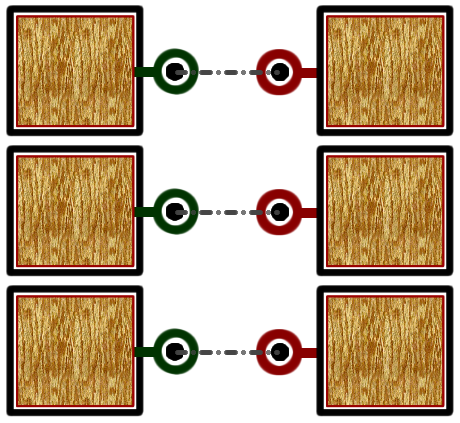
\includegraphics[width=0.25\columnwidth]{comm_11.png}
}
\hspace{0.05\textwidth}%
\subfloat[][Communication 1 à N]{%
	\label{res_subfig:comm_diff}
	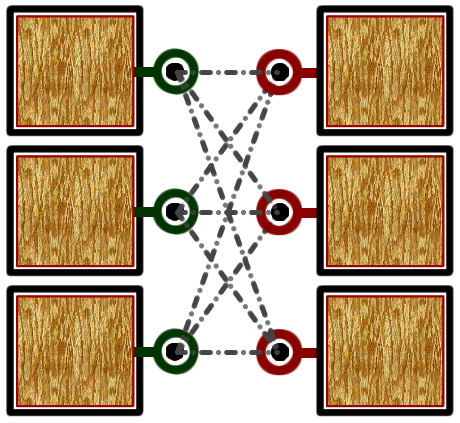
\includegraphics[width=0.25\columnwidth]{comm_1n.png}
}
\caption[]{Représentation graphique des opérateurs de communication}
\label{res_fig:comm}
\end{figure}